\documentclass{standalone}
\usepackage{tikz}
\usetikzlibrary{patterns, positioning}


\begin{document}
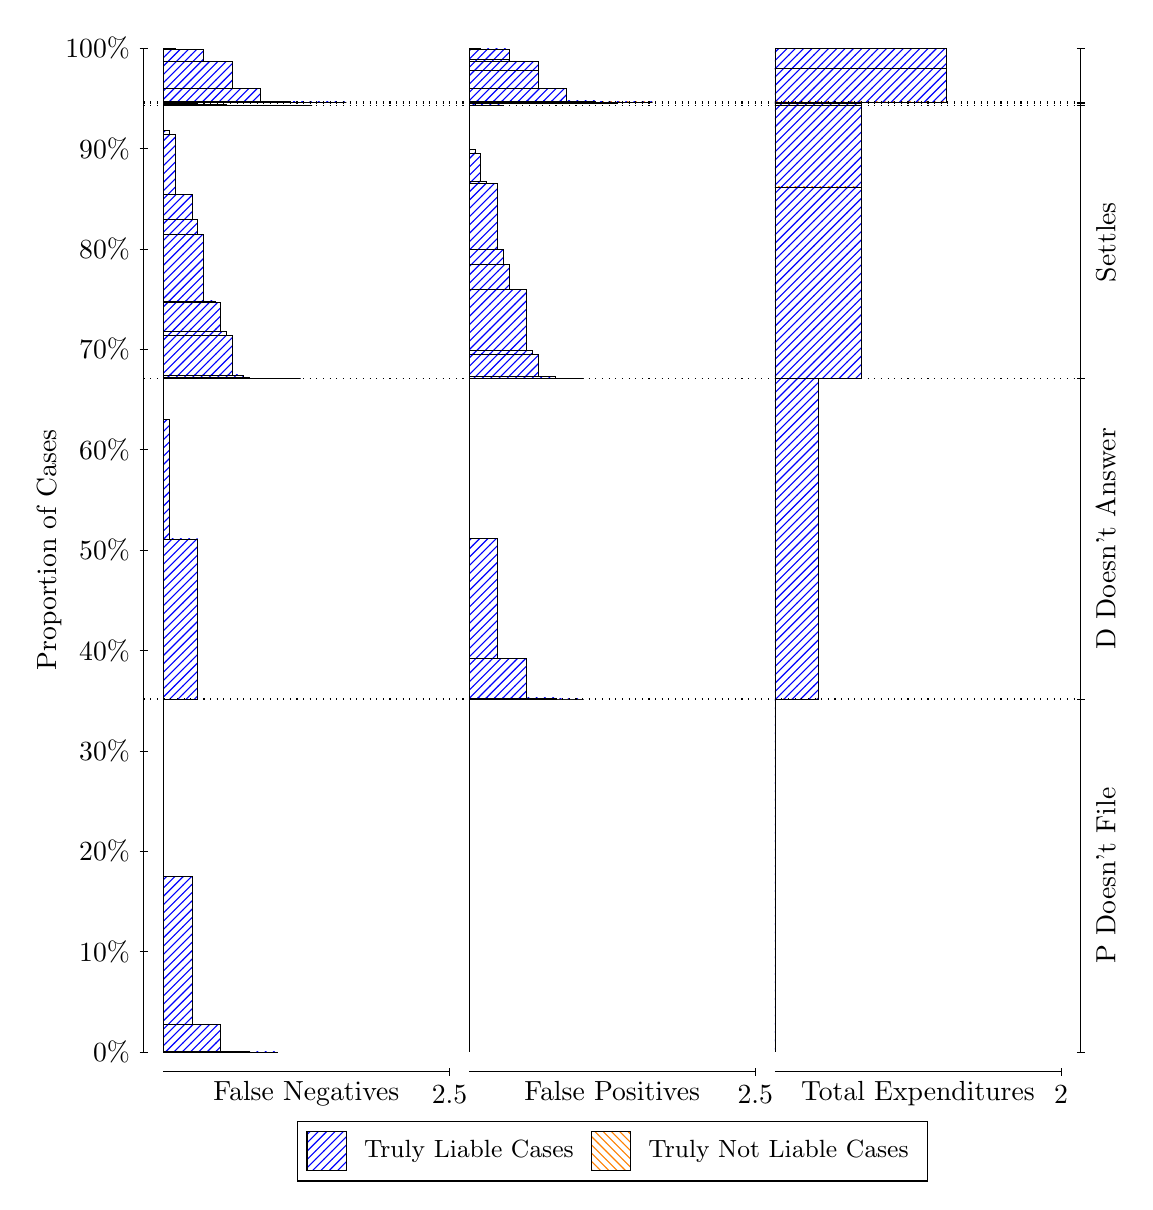
\begin{tikzpicture}
\draw[black, very thin] (1.5,1.75) -- (1.5,14.5);
\node[rotate=90, text=black, anchor=center] at (0.3, 8.125) {Proportion of Cases};
\draw[black, very thin] (1.45,1.75) -- (1.55,1.75);
\node[text=black, anchor=east] at (1.45, 1.75) {0\%};
\draw[black, very thin] (1.45,3.025) -- (1.55,3.025);
\node[text=black, anchor=east] at (1.45, 3.025) {10\%};
\draw[black, very thin] (1.45,4.3) -- (1.55,4.3);
\node[text=black, anchor=east] at (1.45, 4.3) {20\%};
\draw[black, very thin] (1.45,5.575) -- (1.55,5.575);
\node[text=black, anchor=east] at (1.45, 5.575) {30\%};
\draw[black, very thin] (1.45,6.85) -- (1.55,6.85);
\node[text=black, anchor=east] at (1.45, 6.85) {40\%};
\draw[black, very thin] (1.45,8.125) -- (1.55,8.125);
\node[text=black, anchor=east] at (1.45, 8.125) {50\%};
\draw[black, very thin] (1.45,9.4) -- (1.55,9.4);
\node[text=black, anchor=east] at (1.45, 9.4) {60\%};
\draw[black, very thin] (1.45,10.675) -- (1.55,10.675);
\node[text=black, anchor=east] at (1.45, 10.675) {70\%};
\draw[black, very thin] (1.45,11.95) -- (1.55,11.95);
\node[text=black, anchor=east] at (1.45, 11.95) {80\%};
\draw[black, very thin] (1.45,13.225) -- (1.55,13.225);
\node[text=black, anchor=east] at (1.45, 13.225) {90\%};
\draw[black, very thin] (1.45,14.5) -- (1.55,14.5);
\node[text=black, anchor=east] at (1.45, 14.5) {100\%};

\draw[black, very thin] (13.4,1.75) -- (13.4,14.5);
\draw[black, very thin] (13.35,1.75) -- (13.45,1.75);
\node[anchor=west] at (13.35, 1.75) {};
\draw[black, very thin] (13.35,6.2328) -- (13.45,6.2328);
\node[anchor=west] at (13.35, 6.2328) {};
\draw[black, very thin] (13.35,10.302) -- (13.45,10.302);
\node[anchor=west] at (13.35, 10.302) {};
\draw[black, very thin] (13.35,13.769) -- (13.45,13.769);
\node[anchor=west] at (13.35, 13.769) {};
\draw[black, very thin] (13.35,13.796) -- (13.45,13.796);
\node[anchor=west] at (13.35, 13.796) {};
\draw[black, very thin] (13.35,13.815) -- (13.45,13.815);
\node[anchor=west] at (13.35, 13.815) {};
\draw[black, very thin] (13.35,14.5) -- (13.45,14.5);
\node[anchor=west] at (13.35, 14.5) {};

\draw[black, very thin, pattern color=blue, pattern=north east lines] (1.75,1.75) rectangle (3.2033,1.75);
\draw[black, very thin, pattern color=blue, pattern=north east lines] (1.75,1.75) rectangle (2.84,1.753);
\draw[black, very thin, pattern color=blue, pattern=north east lines] (1.75,1.753) rectangle (2.4767,2.1051);
\draw[black, very thin, pattern color=blue, pattern=north east lines] (1.75,2.1051) rectangle (2.1133,3.9787);
\draw[black, very thin, pattern color=orange, pattern=north west lines] (1.75,3.9787) rectangle (1.75,3.9787);
\draw[black, very thin, pattern color=blue, pattern=north east lines] (1.75,3.9787) rectangle (1.75,6.2328);
\draw[black, very thin, pattern color=blue, pattern=north east lines] (1.75,6.2328) rectangle (2.186,8.2661);
\draw[black, very thin, pattern color=blue, pattern=north east lines] (1.75,8.2661) rectangle (1.8227,9.7876);
\draw[black, very thin, pattern color=orange, pattern=north west lines] (1.75,9.7876) rectangle (1.75,9.7876);
\draw[black, very thin, pattern color=blue, pattern=north east lines] (1.75,9.7876) rectangle (1.75,10.302);
\draw[black, very thin, pattern color=blue, pattern=north east lines] (1.75,10.302) rectangle (3.494,10.302);
\draw[black, very thin, pattern color=blue, pattern=north east lines] (1.75,10.302) rectangle (3.2033,10.302);
\draw[black, very thin, pattern color=blue, pattern=north east lines] (1.75,10.302) rectangle (3.1307,10.302);
\draw[black, very thin, pattern color=blue, pattern=north east lines] (1.75,10.302) rectangle (2.9127,10.304);
\draw[black, very thin, pattern color=blue, pattern=north east lines] (1.75,10.304) rectangle (2.84,10.318);
\draw[black, very thin, pattern color=blue, pattern=north east lines] (1.75,10.318) rectangle (2.7673,10.348);
\draw[black, very thin, pattern color=blue, pattern=north east lines] (1.75,10.348) rectangle (2.622,10.855);
\draw[black, very thin, pattern color=blue, pattern=north east lines] (1.75,10.855) rectangle (2.5493,10.905);
\draw[black, very thin, pattern color=blue, pattern=north east lines] (1.75,10.905) rectangle (2.4767,11.267);
\draw[black, very thin, pattern color=blue, pattern=north east lines] (1.75,11.267) rectangle (2.404,11.29);
\draw[black, very thin, pattern color=blue, pattern=north east lines] (1.75,11.29) rectangle (2.2587,12.132);
\draw[black, very thin, pattern color=blue, pattern=north east lines] (1.75,12.132) rectangle (2.186,12.322);
\draw[black, very thin, pattern color=blue, pattern=north east lines] (1.75,12.322) rectangle (2.1133,12.64);
\draw[black, very thin, pattern color=blue, pattern=north east lines] (1.75,12.64) rectangle (2.0407,12.641);
\draw[black, very thin, pattern color=blue, pattern=north east lines] (1.75,12.641) rectangle (1.8953,13.408);
\draw[black, very thin, pattern color=blue, pattern=north east lines] (1.75,13.408) rectangle (1.8227,13.456);
\draw[black, very thin, pattern color=orange, pattern=north west lines] (1.75,13.456) rectangle (1.75,13.456);
\draw[black, very thin, pattern color=blue, pattern=north east lines] (1.75,13.456) rectangle (1.75,13.769);
\draw[black, very thin, pattern color=blue, pattern=north east lines] (1.75,13.769) rectangle (3.6393,13.769);
\draw[black, very thin, pattern color=blue, pattern=north east lines] (1.75,13.769) rectangle (3.276,13.769);
\draw[black, very thin, pattern color=blue, pattern=north east lines] (1.75,13.769) rectangle (2.9127,13.77);
\draw[black, very thin, pattern color=blue, pattern=north east lines] (1.75,13.77) rectangle (2.5493,13.788);
\draw[black, very thin, pattern color=blue, pattern=north east lines] (1.75,13.788) rectangle (2.186,13.796);
\draw[black, very thin, pattern color=orange, pattern=north west lines] (1.75,13.796) rectangle (1.75,13.796);
\draw[black, very thin, pattern color=blue, pattern=north east lines] (1.75,13.796) rectangle (2.186,13.804);
\draw[black, very thin, pattern color=blue, pattern=north east lines] (1.75,13.804) rectangle (1.8227,13.815);
\draw[black, very thin, pattern color=orange, pattern=north west lines] (1.75,13.815) rectangle (1.75,13.815);
\draw[black, very thin, pattern color=blue, pattern=north east lines] (1.75,13.815) rectangle (1.75,13.815);
\draw[black, very thin, pattern color=blue, pattern=north east lines] (1.75,13.815) rectangle (4.0753,13.815);
\draw[black, very thin, pattern color=blue, pattern=north east lines] (1.75,13.815) rectangle (3.712,13.815);
\draw[black, very thin, pattern color=blue, pattern=north east lines] (1.75,13.815) rectangle (3.3487,13.826);
\draw[black, very thin, pattern color=blue, pattern=north east lines] (1.75,13.826) rectangle (2.9853,13.984);
\draw[black, very thin, pattern color=blue, pattern=north east lines] (1.75,13.984) rectangle (2.622,14.328);
\draw[black, very thin, pattern color=blue, pattern=north east lines] (1.75,14.328) rectangle (2.2587,14.487);
\draw[black, very thin, pattern color=blue, pattern=north east lines] (1.75,14.487) rectangle (1.8953,14.5);
\draw[black, very thin, pattern color=orange, pattern=north west lines] (1.75,14.5) rectangle (1.75,14.5);
\draw[black, very thin, pattern color=blue, pattern=north east lines] (1.75,14.5) rectangle (1.75,14.5);
\draw[black, very thin, pattern color=orange, pattern=north west lines] (5.6333,1.75) rectangle (5.6333,1.75);
\draw[black, very thin, pattern color=blue, pattern=north east lines] (5.6333,1.75) rectangle (5.6333,6.2328);
\draw[black, very thin, pattern color=orange, pattern=north west lines] (5.6333,6.2328) rectangle (7.0867,6.2328);
\draw[black, very thin, pattern color=blue, pattern=north east lines] (5.6333,6.2328) rectangle (7.0867,6.2328);
\draw[black, very thin, pattern color=blue, pattern=north east lines] (5.6333,6.2328) rectangle (6.7233,6.2455);
\draw[black, very thin, pattern color=blue, pattern=north east lines] (5.6333,6.2455) rectangle (6.36,6.7469);
\draw[black, very thin, pattern color=blue, pattern=north east lines] (5.6333,6.7469) rectangle (5.9967,8.2684);
\draw[black, very thin, pattern color=blue, pattern=north east lines] (5.6333,8.2684) rectangle (5.6333,10.302);
\draw[black, very thin, pattern color=orange, pattern=north west lines] (5.6333,10.302) rectangle (7.0867,10.302);
\draw[black, very thin, pattern color=blue, pattern=north east lines] (5.6333,10.302) rectangle (7.0867,10.302);
\draw[black, very thin, pattern color=orange, pattern=north west lines] (5.6333,10.302) rectangle (6.796,10.302);
\draw[black, very thin, pattern color=blue, pattern=north east lines] (5.6333,10.302) rectangle (6.796,10.303);
\draw[black, very thin, pattern color=blue, pattern=north east lines] (5.6333,10.303) rectangle (6.7233,10.331);
\draw[black, very thin, pattern color=orange, pattern=north west lines] (5.6333,10.331) rectangle (6.5053,10.331);
\draw[black, very thin, pattern color=blue, pattern=north east lines] (5.6333,10.331) rectangle (6.5053,10.615);
\draw[black, very thin, pattern color=blue, pattern=north east lines] (5.6333,10.615) rectangle (6.4327,10.663);
\draw[black, very thin, pattern color=blue, pattern=north east lines] (5.6333,10.663) rectangle (6.36,11.43);
\draw[black, very thin, pattern color=orange, pattern=north west lines] (5.6333,11.43) rectangle (6.2147,11.43);
\draw[black, very thin, pattern color=blue, pattern=north east lines] (5.6333,11.43) rectangle (6.2147,11.43);
\draw[black, very thin, pattern color=blue, pattern=north east lines] (5.6333,11.43) rectangle (6.142,11.749);
\draw[black, very thin, pattern color=blue, pattern=north east lines] (5.6333,11.749) rectangle (6.0693,11.939);
\draw[black, very thin, pattern color=blue, pattern=north east lines] (5.6333,11.939) rectangle (5.9967,12.781);
\draw[black, very thin, pattern color=blue, pattern=north east lines] (5.6333,12.781) rectangle (5.8513,12.804);
\draw[black, very thin, pattern color=blue, pattern=north east lines] (5.6333,12.804) rectangle (5.7787,13.165);
\draw[black, very thin, pattern color=blue, pattern=north east lines] (5.6333,13.165) rectangle (5.706,13.216);
\draw[black, very thin, pattern color=blue, pattern=north east lines] (5.6333,13.216) rectangle (5.6333,13.769);
\draw[black, very thin, pattern color=orange, pattern=north west lines] (5.6333,13.769) rectangle (6.0693,13.769);
\draw[black, very thin, pattern color=blue, pattern=north east lines] (5.6333,13.769) rectangle (6.0693,13.777);
\draw[black, very thin, pattern color=blue, pattern=north east lines] (5.6333,13.777) rectangle (5.706,13.795);
\draw[black, very thin, pattern color=blue, pattern=north east lines] (5.6333,13.795) rectangle (5.6333,13.796);
\draw[black, very thin, pattern color=orange, pattern=north west lines] (5.6333,13.796) rectangle (7.5227,13.796);
\draw[black, very thin, pattern color=blue, pattern=north east lines] (5.6333,13.796) rectangle (7.5227,13.796);
\draw[black, very thin, pattern color=blue, pattern=north east lines] (5.6333,13.796) rectangle (7.1593,13.796);
\draw[black, very thin, pattern color=blue, pattern=north east lines] (5.6333,13.796) rectangle (6.796,13.796);
\draw[black, very thin, pattern color=blue, pattern=north east lines] (5.6333,13.796) rectangle (6.4327,13.808);
\draw[black, very thin, pattern color=blue, pattern=north east lines] (5.6333,13.808) rectangle (6.0693,13.815);
\draw[black, very thin, pattern color=orange, pattern=north west lines] (5.6333,13.815) rectangle (7.9587,13.815);
\draw[black, very thin, pattern color=blue, pattern=north east lines] (5.6333,13.815) rectangle (7.9587,13.815);
\draw[black, very thin, pattern color=orange, pattern=north west lines] (5.6333,13.815) rectangle (7.5953,13.815);
\draw[black, very thin, pattern color=blue, pattern=north east lines] (5.6333,13.815) rectangle (7.5953,13.815);
\draw[black, very thin, pattern color=orange, pattern=north west lines] (5.6333,13.815) rectangle (7.232,13.815);
\draw[black, very thin, pattern color=blue, pattern=north east lines] (5.6333,13.815) rectangle (7.232,13.828);
\draw[black, very thin, pattern color=blue, pattern=north east lines] (5.6333,13.828) rectangle (6.8687,13.987);
\draw[black, very thin, pattern color=orange, pattern=north west lines] (5.6333,13.987) rectangle (6.8687,13.987);
\draw[black, very thin, pattern color=blue, pattern=north east lines] (5.6333,13.987) rectangle (6.8687,13.987);
\draw[black, very thin, pattern color=blue, pattern=north east lines] (5.6333,13.987) rectangle (6.5053,14.214);
\draw[black, very thin, pattern color=orange, pattern=north west lines] (5.6333,14.214) rectangle (6.5053,14.214);
\draw[black, very thin, pattern color=blue, pattern=north east lines] (5.6333,14.214) rectangle (6.5053,14.331);
\draw[black, very thin, pattern color=blue, pattern=north east lines] (5.6333,14.331) rectangle (6.142,14.357);
\draw[black, very thin, pattern color=blue, pattern=north east lines] (5.6333,14.357) rectangle (6.142,14.49);
\draw[black, very thin, pattern color=blue, pattern=north east lines] (5.6333,14.49) rectangle (5.7787,14.49);
\draw[black, very thin, pattern color=blue, pattern=north east lines] (5.6333,14.49) rectangle (5.7787,14.5);
\draw[black, very thin, pattern color=blue, pattern=north east lines] (5.6333,14.5) rectangle (5.6333,14.5);
\draw[black, very thin, pattern color=orange, pattern=north west lines] (9.5167,1.75) rectangle (9.5167,1.75);
\draw[black, very thin, pattern color=blue, pattern=north east lines] (9.5167,1.75) rectangle (9.5167,6.2328);
\draw[black, very thin, pattern color=orange, pattern=north west lines] (9.5167,6.2328) rectangle (10.062,6.2328);
\draw[black, very thin, pattern color=blue, pattern=north east lines] (9.5167,6.2328) rectangle (10.062,10.302);
\draw[black, very thin, pattern color=orange, pattern=north west lines] (9.5167,10.302) rectangle (10.607,10.302);
\draw[black, very thin, pattern color=blue, pattern=north east lines] (9.5167,10.302) rectangle (10.607,12.737);
\draw[black, very thin, pattern color=orange, pattern=north west lines] (9.5167,12.737) rectangle (10.607,12.737);
\draw[black, very thin, pattern color=blue, pattern=north east lines] (9.5167,12.737) rectangle (10.607,13.769);
\draw[black, very thin, pattern color=orange, pattern=north west lines] (9.5167,13.769) rectangle (10.607,13.769);
\draw[black, very thin, pattern color=blue, pattern=north east lines] (9.5167,13.769) rectangle (10.607,13.796);
\draw[black, very thin, pattern color=orange, pattern=north west lines] (9.5167,13.796) rectangle (10.607,13.796);
\draw[black, very thin, pattern color=blue, pattern=north east lines] (9.5167,13.796) rectangle (10.607,13.815);
\draw[black, very thin, pattern color=orange, pattern=north west lines] (9.5167,13.815) rectangle (11.697,13.815);
\draw[black, very thin, pattern color=blue, pattern=north east lines] (9.5167,13.815) rectangle (11.697,14.238);
\draw[black, very thin, pattern color=orange, pattern=north west lines] (9.5167,14.238) rectangle (11.697,14.238);
\draw[black, very thin, pattern color=blue, pattern=north east lines] (9.5167,14.238) rectangle (11.697,14.5);
\draw[black, dotted] (1.5,6.2328) -- (13.4,6.2328);
\draw[black, dotted] (1.5,10.302) -- (13.4,10.302);
\draw[black, dotted] (1.5,13.769) -- (13.4,13.769);
\draw[black, dotted] (1.5,13.796) -- (13.4,13.796);
\draw[black, dotted] (1.5,13.815) -- (13.4,13.815);
\draw[black, very thin] (1.75,1.5) -- (5.3833,1.5);
\node[text=black, anchor=north] at (3.5667, 1.5) {False Negatives};
\draw[black, very thin] (5.3833,1.45) -- (5.3833,1.55);
\node[text=black, anchor=north] at (5.3833, 1.45) {2.5};

\draw[black, very thin] (5.6333,1.5) -- (9.2667,1.5);
\node[text=black, anchor=north] at (7.45, 1.5) {False Positives};
\draw[black, very thin] (9.2667,1.45) -- (9.2667,1.55);
\node[text=black, anchor=north] at (9.2667, 1.45) {2.5};

\draw[black, very thin] (9.5167,1.5) -- (13.15,1.5);
\node[text=black, anchor=north] at (11.333, 1.5) {Total Expenditures};
\draw[black, very thin] (13.15,1.45) -- (13.15,1.55);
\node[text=black, anchor=north] at (13.15, 1.45) {2};

\node[text=black, centered, rotate=90] at (13.72, 3.9914) {P Doesn't File};
\node[text=black, centered, rotate=90] at (13.72, 8.2673) {D Doesn't Answer};
\node[text=black, centered, rotate=90] at (13.72, 12.035) {Settles};




\draw (7.449999999999999,1.5) node[draw=none] (baseCoordinate) {};
\begin{scope}[align=center]
        \matrix[scale=0.5, draw=black, below=0.5cm of baseCoordinate, nodes={draw}, column sep=0.1cm]{
            \node[rectangle, draw, minimum width=0.5cm, minimum height=0.5cm, pattern color=blue, pattern=north east lines] {}; &
            \node[draw=none, font=\small, text=black] (B) {Truly Liable Cases}; &
            \node[rectangle, draw, minimum width=0.5cm, minimum height=0.5cm, pattern color=orange, pattern=north west lines] {}; &
            \node[draw=none, font=\small, text=black] (B) {Truly Not Liable Cases}; \\
            };
\end{scope}

\end{tikzpicture}
\end{document}